%%
%% This is file `sample-manuscript.tex',
%% generated with the docstrip utility.
%%
%% The original source files were:
%%
%% samples.dtx  (with options: `all,proceedings,bibtex,manuscript')
%% 
%% IMPORTANT NOTICE:
%% 
%% For the copyright see the source file.
%% 
%% Any modified versions of this file must be renamed
%% with new filenames distinct from sample-manuscript.tex.
%% 
%% For distribution of the original source see the terms
%% for copying and modification in the file samples.dtx.
%% 
%% This generated file may be distributed as long as the
%% original source files, as listed above, are part of the
%% same distribution. (The sources need not necessarily be
%% in the same archive or directory.)
%%
%%
%% Commands for TeXCount
%TC:macro \cite [option:text,text]
%TC:macro \citep [option:text,text]
%TC:macro \citet [option:text,text]
%TC:envir table 0 1
%TC:envir table* 0 1
%TC:envir tabular [ignore] word
%TC:envir displaymath 0 word
%TC:envir math 0 word
%TC:envir comment 0 0
%%
%% The first command in your LaTeX source must be the \documentclass
%% command.
%%
%% For submission and review of your manuscript please change the
%% command to \documentclass[manuscript, screen, review]{acmart}.
%%
%% When submitting camera ready or to TAPS, please change the command
%% to \documentclass[sigconf]{acmart} or whichever template is required
%% for your publication.
%%
%%
\documentclass[manuscript,screen,review]{acmart}
\usepackage{indentfirst} % 必须添加
%%
%% \BibTeX command to typeset BibTeX logo in the docs
\AtBeginDocument{%
  \providecommand\BibTeX{{%
    Bib\TeX}}}

%% Rights management information.  This information is sent to you
%% when you complete the rights form.  These commands have SAMPLE
%% values in them; it is your responsibility as an author to replace
%% the commands and values with those provided to you when you
%% complete the rights form.
\setcopyright{acmlicensed}
\copyrightyear{2018}
\acmYear{2018}
\acmDOI{XXXXXXX.XXXXXXX}
%% These commands are for a PROCEEDINGS abstract or paper.
\acmConference[Conference acronym 'XX]{Make sure to enter the correct
  conference title from your rights confirmation email}{June 03--05,
  2018}{Woodstock, NY}
%%
%%  Uncomment \acmBooktitle if the title of the proceedings is different
%%  from ``Proceedings of ...''!
%%
%%\acmBooktitle{Woodstock '18: ACM Symposium on Neural Gaze Detection,
%%  June 03--05, 2018, Woodstock, NY}
\acmISBN{978-1-4503-XXXX-X/2018/06}


%%
%% Submission ID.
%% Use this when submitting an article to a sponsored event. You'll
%% receive a unique submission ID from the organizers
%% of the event, and this ID should be used as the parameter to this command.
%%\acmSubmissionID{123-A56-BU3}

%%
%% For managing citations, it is recommended to use bibliography
%% files in BibTeX format.
%%
%% You can then either use BibTeX with the ACM-Reference-Format style,
%% or BibLaTeX with the acmnumeric or acmauthoryear sytles, that include
%% support for advanced citation of software artefact from the
%% biblatex-software package, also separately available on CTAN.
%%
%% Look at the sample-*-biblatex.tex files for templates showcasing
%% the biblatex styles.
%%

%%
%% The majority of ACM publications use numbered citations and
%% references.  The command \citestyle{authoryear} switches to the
%% "author year" style.
%%
%% If you are preparing content for an event
%% sponsored by ACM SIGGRAPH, you must use the "author year" style of
%% citations and references.
%% Uncommenting
%% the next command will enable that style.
%%\citestyle{acmauthoryear}


%%
%% end of the preamble, start of the body of the document source.
\begin{document}

%%
%% The "title" command has an optional parameter,
%% allowing the author to define a "short title" to be used in page headers.
\title{The Name of the Title Is Hope}

%%
%% The "author" command and its associated commands are used to define
%% the authors and their affiliations.
%% Of note is the shared affiliation of the first two authors, and the
%% "authornote" and "authornotemark" commands
%% used to denote shared contribution to the research.
\author{Zheng Li}
\authornote{Both authors contributed equally to this research.}
\affiliation{
  \institution{Southeast University}
  \city{Nanjing}
  \country{China}
}
\email{LiZheng040910@163.com}

%%
%% By default, the full list of authors will be used in the page
%% headers. Often, this list is too long, and will overlap
%% other information printed in the page headers. This command allows
%% the author to define a more concise list
%% of authors' names for this purpose.
\renewcommand{\shortauthors}{Trovato et al.}

%%
%% The abstract is a short summary of the work to be presented in the
%% article.
\begin{abstract}

\end{abstract}

%%
%% The code below is generated by the tool at http://dl.acm.org/ccs.cfm.
%% Please copy and paste the code instead of the example below.
%%
% \begin{CCSXML}
% <ccs2012>
%  <concept>
%   <concept_id>00000000.0000000.0000000</concept_id>
%   <concept_desc>Do Not Use This Code, Generate the Correct Terms for Your Paper</concept_desc>
%   <concept_significance>500</concept_significance>
%  </concept>
%  <concept>
%   <concept_id>00000000.00000000.00000000</concept_id>
%   <concept_desc>Do Not Use This Code, Generate the Correct Terms for Your Paper</concept_desc>
%   <concept_significance>300</concept_significance>
%  </concept>
%  <concept>
%   <concept_id>00000000.00000000.00000000</concept_id>
%   <concept_desc>Do Not Use This Code, Generate the Correct Terms for Your Paper</concept_desc>
%   <concept_significance>100</concept_significance>
%  </concept>
%  <concept>
%   <concept_id>00000000.00000000.00000000</concept_id>
%   <concept_desc>Do Not Use This Code, Generate the Correct Terms for Your Paper</concept_desc>
%   <concept_significance>100</concept_significance>
%  </concept>
% </ccs2012>
% \end{CCSXML}

% \ccsdesc[500]{Do Not Use This Code~Generate the Correct Terms for Your Paper}
% \ccsdesc[300]{Do Not Use This Code~Generate the Correct Terms for Your Paper}
% \ccsdesc{Do Not Use This Code~Generate the Correct Terms for Your Paper}
% \ccsdesc[100]{Do Not Use This Code~Generate the Correct Terms for Your Paper}

%%
%% Keywords. The author(s) should pick words that accurately describe
%% the work being presented. Separate the keywords with commas.
\keywords{Do, Not, Us, This, Code, Put, the, Correct, Terms, for,
  Your, Paper}
%%
%% This command processes the author and affiliation and title
%% information and builds the first part of the formatted document.
\maketitle

\section{Introduction}

\subsection{Motivation of AI in Software Testing}

\subsection{AI as a Tool for Testing Traditional Systems}

\section{AI-Driven Test Data Generation}

\subsection{Data Augmentations for Edge Cases}

\subsection{Generative AI for Synthetic Data}

\subsection{Adversarial Sample Generation}

\section{AI-Powered Test Case Optimization}
\label{sec:3}

This chapter will detail how to leverage artificial intelligence techniques in software testing, specifically focusing on optimization methods based on Boundary Coverage Distance (BCD) and techniques using Reinforcement Learning (RL), to achieve intelligent test case generation and boundary exploration. First, in the introduction, we present the background and significance of this chapter. Then, this section is divided into two core subsections, which respectively introduce BCD-optimized boundary value analysis and the application of reinforcement learning in test exploration. Finally, we summarize and prospect the content of this chapter.

As software systems become increasingly complex and the requirements for reliability and safety continue to rise, traditional test case design methods that rely on manual experience can no longer meet practical needs. On one hand, traditional equivalence class partitioning and Boundary Value Analysis (BVA) methods, when facing high-dimensional and multi-branch complex software, require manual extraction of a large number of boundary conditions, which is extremely challenging and inefficient. On the other hand, Random Testing (RT) and Adaptive Random Testing (ART), although able to improve test coverage to some extent, still lack exploration capability for boundary defects. Therefore, how to maximize the coverage of potential boundary defect areas in software while ensuring test efficiency has become a pressing challenge in the field of software engineering.

AI-driven test case optimization emerges in this context. On one hand, by quantifying the boundary coverage with a metric like Boundary Coverage Distance (BCD), test case design can be transformed into an optimization problem, allowing intelligent algorithms to automatically search for optimal test points in the input domain. On the other hand, intelligent techniques such as reinforcement learning can dynamically construct environments and testing strategies, interacting with the system under test to efficiently approach failure boundaries and uncover defects in extreme scenarios. Combining both approaches not only reduces the manual workload of testers but also achieves more comprehensive and precise boundary testing in high-dimensional complex scenarios.

This chapter aims to clarify the principles and application effects of two main AI-driven methods for test case generation and boundary exploration. First, we will delve into BCD-based boundary value analysis, including the mathematical definition of BCD, its computation method, and the implementation of test case auto-generation using MCMC (Markov Chain Monte Carlo) optimization strategies. Then, considering dynamic scenarios such as autonomous driving, we will discuss the advantages of reinforcement learning in test exploration, emphasizing the necessity of dynamic threshold design in the boundary approach process. By citing real experimental results and visualization examples from the literature, we demonstrate the significant improvements in defect detection rates and efficiency provided by these two approaches. Finally, we offer a summary of this chapter and look forward to future integrations of AI and software testing.
\subsection{Boundary Value Analysis with BCD Optimization}

Before formally introducing BCD, let us first review the basic idea of Boundary Value Analysis (BVA). BVA is a black-box testing technique based on the experience that ``system defects often occur near boundary conditions. Its core is to select values near partition boundaries in the input domain to construct test cases, aiming to identify ``off-by-one errors or ``boundary omissions.'' However, traditional BVA often relies on testers manually identifying equivalence partitions and corresponding boundaries based on requirement documents. For software systems with high-dimensional input domains and complex constraint relationships, this manual approach is time-consuming and prone to omissions.

To address the insufficient coverage by manually selecting boundary values, Guo \textit{et al.}\cite{Guo2024} proposed a metric called \textbf{Boundary Coverage Distance (BCD)} and, based on this, designed a test case optimization algorithm using MCMC. Compared to traditional BVA, which only focuses on ``whether a boundary is hit,'' BCD introduces an integer distance metric that measures the minimum distance between test cases and all boundary points, thus transforming the boundary coverage problem into an optimization problem. This metric can reflect the distribution of the test suite across the entire boundary space and supports the automated generation of optimal test cases.

First, we provide the mathematical definitions of equivalence partitions and boundaries. Let the input domain of the software under test be $I$, and the output domain be $O = f(I)$. We divide the output into $m$ mutually disjoint categories: $O = \bigcup_{i=1}^m O_i$, with $O_i \cap O_j = \emptyset$ for $i \neq j$. Correspondingly, define the input equivalence partitions:
\begin{equation}
I_i := \{\, x \in I \mid f(x) \in O_i \,\}, \quad i = 1,2,\ldots,m. \tag{1}
\end{equation}
Any input $x \in I$ yields an output that belongs to some category $O_i$, so $x$ belongs to the corresponding equivalence partition $I_i$. Within this framework, we need to clarify the minimal unit of ``input change.'' Let $G$ be a set of functions satisfying the following properties:
\begin{enumerate}
  \item For any $g \in G$, its inverse operation $g^{-1}$ also belongs to $G$.
  \item For any $x,y \in I$, there exists a finite sequence of operations $\{g_1, g_2, \ldots, g_n\} \subset G$ such that $y = g_1 \circ g_2 \circ \cdots \circ g_n(x)$.
\end{enumerate}
A function $g \in G$ is called a ``minimal operation'' on the input, and having its inverse ensures reversibility. Then, define the boundary set of the equivalence partition $I_i$ as:
\begin{equation}
B_i := \bigl\{\, x \in I_i \mid \exists\, g \in G,\ f\bigl(g(x)\bigr) \notin O_i \bigr\}. \tag{2}
\end{equation}
In other words, if an input $x$ belongs to $I_i$, but applying a minimal operation to it causes it to leave the equivalence partition $I_i$, then $x$ is considered a boundary point. Geometrically, $B_i$ lies on the boundary between $I_i$ and other equivalence partitions.

Next, we introduce the distance measure between test inputs and boundary points. Let $d(x,y)$ denote the number of minimal operations needed to go from input $x$ to input $y$, i.e.,
\begin{equation}
d(x,y) \;=\; \min\bigl\{\, n \ge 0 \mid y = g_n \circ g_{n-1} \circ \cdots \circ g_1(x),\ g_j \in G \bigr\}. \tag{3}
\end{equation}
For example, in the ``English exam grading'' example, if $G = \{\, g_1:\text{Listening}+1,\ g_2:\text{Listening}-1,\ g_3:\text{Reading}+1,\ g_4:\text{Reading}-1 \,\}$, then going from input $x = (-1,-1)$ to $y=(0,0)$ requires two steps (apply $g_1$ then $g_3$), so $d((-1,-1),(0,0)) = 2$.

Let the test set for an equivalence partition $I_i$ be $T_i \subseteq I_i$. To measure how well $T_i$ covers its boundary $B_i$, we compute for each boundary point $y \in B_i$ the minimum distance to any test point in $T_i$ and then take the maximum over all $y$:
\begin{equation}
d\bigl(T_i,\, B_i \bigr) \;=\; \max_{y \in B_i} \; \min_{x \in T_i} d(x,y). \tag{4}
\end{equation}
If $T_i$ is empty, define $d(T_i,B_i) = +\infty$. Intuitively, equation (4) first finds the closest test point to each boundary point, then the worst-case distance over all boundary points, reflecting the ``weakest'' boundary coverage. Finally, let the overall test set be $T = \bigcup_{i=1}^m T_i$ and the union of all boundary sets $B = \bigcup_{i=1}^m B_i$. We define the overall boundary coverage distance as:
\begin{equation}
\mathrm{BCD}(T) \;=\; d(T,B) \;=\; \max_{i=1,\ldots,m}\; d\bigl(T_i,\, B_i\bigr). \tag{5}
\end{equation}
When $\mathrm{BCD}(T) = 0$, the test set $T$ covers every boundary point in all partitions. Conversely, if $\mathrm{BCD}(T) = k > 0$, there exists some partition whose boundary point is at distance $k$ from the nearest test point, indicating incomplete boundary coverage.

With BCD as a metric, test case generation becomes a \emph{BCD minimization} problem: given a fixed number of test cases $n$, how do we select or optimize an initial test set $T$ to minimize $\mathrm{BCD}(T)$? To solve this optimization problem, Guo \textit{et al.}\cite{Guo2024} borrow ideas from the Markov Chain Monte Carlo (MCMC) algorithm and propose three main test input generation and optimization strategies, referred to as \textbf{Algorithm~1}, \textbf{Algorithm~2}, and \textbf{Algorithm~3}. Below is a brief introduction to the core ideas and implementation steps of these algorithms.

\paragraph{Algorithm 1: Greedy Descent BCD Optimization}  
Algorithm 1 first \emph{randomly} generates $n$ initial test points in the input domain, forming the set $T = \{\, t_1, t_2, \ldots, t_n \}$. It then iteratively executes the following steps until a preset iteration count is reached or the BCD value converges:
\begin{enumerate}
  \item Compute the current BCD value of the test set $T$, i.e., $\mathrm{BCD}(T)$.
  \item Randomly select a test point $t$ from $T$, and generate a candidate input $t'$ according to a \emph{proposal distribution}. Typically, the proposal distribution perturbs $t$ by adding random changes such as $\{-1, 0, 1\}$ for numerical data; for discrete data, switch to a neighboring state.
  \item Form the candidate test set $T'$, where $t$ is replaced by $t'$. Compute $\mathrm{BCD}(T')$. If $\mathrm{BCD}(T') < \mathrm{BCD}(T)$, \textbf{accept} the candidate and update $T \leftarrow T'$; otherwise, \textbf{reject} it and keep $T$ unchanged.
\end{enumerate}
By repeatedly iterating, the test points gradually shift from a random distribution toward an optimal distribution that spans the boundaries. Because the algorithm only accepts candidates that strictly reduce BCD, Algorithm~1 is essentially a \emph{greedy descent} strategy and can easily become trapped in local optima. To illustrate this process, it is analogous to the Metropolis-Hastings acceptance rule:
\[
P_{\mathrm{accept}} =
\begin{cases}
1, & \mathrm{BCD}(T') < \mathrm{BCD}(T), \\
0, & \text{otherwise}.
\end{cases}
\]
Although simple, this algorithm has been shown in practice to significantly improve boundary coverage of the test set. In the experiment with the English exam grading program, the initial random set of 30 test points had a large BCD. After 10\,000 iterations, all test points approached the boundary lines, resulting in $\mathrm{BCD}(T) = 0$ (meaning every boundary in each partition was directly hit). Correspondingly, the mutation kill rate improved from 36\% for random testing to over 80\%.

\paragraph{Algorithm 2: ``Harmless'' Boundary Improvement Strategy}  
Because Algorithm 1 is too strict—only accepting candidates that reduce BCD—it can easily get stuck in local optima. Algorithm 2 refines the acceptance criterion by introducing the notion of a ``\emph{harmless improvement}'': if a candidate reduces the distance to at least one boundary point and does not increase the distance to any other boundary point, then accept the candidate; otherwise, reject it. Formally:
\begin{enumerate}
  \item Select the current test set $T$, randomly pick a point $t \in T$, and generate a candidate $t'$.
  \item For each partition $I_i$, compare the distance of each boundary point $y \in B_i$ before and after replacement. Let $b_{\mathrm{decrease}}$ be the number of boundary points whose distance decreases under the candidate, and $b_{\mathrm{increase}}$ be the number of boundary points whose distance increases.
  \item If $b_{\mathrm{decrease}} > 0$ and $b_{\mathrm{increase}} = 0$, then accept the candidate ($T \leftarrow T'$); otherwise, reject it.
\end{enumerate}

Since this criterion allows candidates as long as they improve at least one boundary without harming others, it has greater exploratory power than Algorithm 1. Experiments show Algorithm 2 can quickly reduce BCD in the early stages, but later, because it only permits ``non-degrading improvements,'' it may stagnate in some partitions. However, compared to Algorithm 1, Algorithm 2 shows a slight improvement in mutation kill rates for most benchmark programs. For example, on the triType program, Algorithm 1 under the BCD$_{\max}$ metric achieved an 80\% kill rate, while Algorithm 2 improved it to 85\%.

\paragraph{Algorithm 3: Probabilistic Acceptance (MCMC with Temperature)}  
Algorithm 3 further introduces a \emph{probabilistic acceptance} mechanism, allowing a candidate to be accepted with some probability even if it increases certain boundary distances, thus enabling escape from local optima. The detailed steps are:
\begin{enumerate}
  \item As in Algorithm 2, generate the candidate set $T'$ and compute $b_{\mathrm{decrease}}$ and $b_{\mathrm{increase}}$.
  \item If $b_{\mathrm{decrease}} > 0$ and $b_{\mathrm{increase}} = 0$, accept $T'$ unconditionally.
  \item Otherwise, accept $T'$ with probability
  \[
    P_{\mathrm{accept}} = \exp\bigl( -\, (\,b_{\mathrm{increase}} - b_{\mathrm{decrease}}\,)\,/\,T \bigr),
  \]
  where $T$ is the temperature parameter in simulated annealing, which gradually decreases over iterations. If not accepted, reject the candidate.
\end{enumerate}
This strategy balances exploration and exploitation. In the early high-temperature phase, it allows more aggressive exploration by accepting some candidates that slightly increase BCD; as the temperature lowers, only a small number of ``weakly degrading'' candidates are accepted, eventually converging to a better solution. Experimental results demonstrate that Algorithm 3 outperforms Algorithm 2 in avoiding early convergence to local optima, especially in complex programs with uneven boundary distributions (e.g., miniSAT). For instance, in the miniSAT test experiment, Algorithm 2 under BCD$_{i}$ achieved approximately an 85\% kill rate, whereas Algorithm 3 under BCD$_{i}$ improved it to 93\%.

\paragraph{Boundary Distribution for English Exam Grading}  
Figure~\ref{fig:english_boundary} shows the basic boundary distribution of the English exam grading program on the two-dimensional input plane. In this figure, the gray region represents invalid inputs ($I_1$), the blue region represents ``fail'' ($I_3$), and the orange region represents ``pass'' ($I_2$). The dashed black lines depict the equivalence partition boundaries as defined by equations (3)-(5). Each boundary corresponds to inputs where a minimal operation can move a score combination from one output category to another. This illustration provides a clear view of how the input domain is partitioned into $I_1$, $I_2$, and $I_3$ and where their shared boundaries lie.

\begin{figure}[htb]
  \centering
  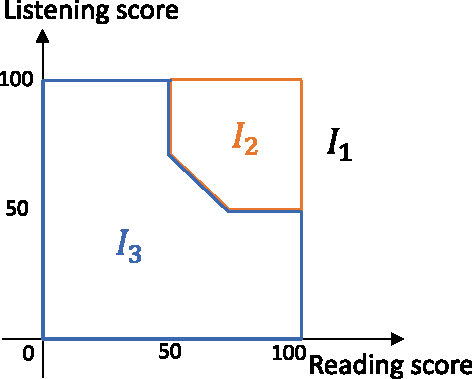
\includegraphics[width=0.5\linewidth]{./picture/1.pdf}
  \caption{Basic boundary distribution for the English exam grading program: gray indicates invalid inputs ($I_1$), blue indicates fail ($I_3$), orange indicates pass ($I_2$), and black dashed lines show the equivalence partition boundaries.}
  \label{fig:english_boundary}
\end{figure}

In the BCD metric experiment, the random test set of 30 points had $\mathrm{BCD} = 5$ (meaning some boundary points were five minimal steps away from the nearest test points), while Algorithm 1 under the BCD$_{\mathrm{mean}}$ criterion reduced $\mathrm{BCD}$ to 0 after 10\,000 iterations, achieving direct coverage of all boundary points. Correspondingly, the mutation kill rate improved from 36\% (random testing) to 80\%. This experimental result fully demonstrates the effectiveness of BCD-based boundary value optimization in black-box testing.
\subsection{Reinforcement Learning for Test Exploration}
Traditional static boundary value analysis methods have inherent limitations when dealing with \textbf{dynamic decision systems}. Take an autonomous driving system as an example: test scenarios are not limited to single-input judgments but involve continuous, multi-round interactions between the system and the environment. Such scenarios typically involve continuous state spaces, high-dimensional action spaces, and uncertain environmental disturbances. Therefore, efficiently generating test sequences that can trigger potential faults or extreme behaviors is challenging. To address this, researchers have introduced \textbf{reinforcement learning} techniques into the domain of software testing. Through interactions between an agent (the RL tester) and the system under test in a simulated environment, the agent actively explores and approaches the system’s failure boundary.

Reinforcement learning-driven test exploration can be broken down into the following core elements: (1) \textbf{state representation}, which abstracts the current system and environment status into features recognizable by the RL agent; (2) \textbf{action space}, representing the controllable interventions the testing agent can apply to the environment or the system under test; (3) \textbf{reward function}, which measures whether the sequence of actions successfully approaches or triggers the failure boundary; and (4) \textbf{policy learning}, whereby the agent continuously interacts with the environment to optimize its policy to achieve the desired goal within a limited number of steps. In the context of autonomous driving testing, the state might include current vehicle speed, distance to the car in front, and road type; the agent’s actions could be accelerate, brake, steer, or introduce environmental disturbances; and the reward function is typically designed as the negative distance to the safety boundary (closer distances receive higher reward), or if a collision occurs, a large positive reward is given to encourage exploration of dangerous scenarios.

\paragraph{Agent-Environment Construction}  
For an autonomous driving control system under test, we can construct the reinforcement learning environment as follows:
\begin{itemize}
  \item \textbf{Environment}: A simulated road scenario, including lanes, curb, obstacles, pedestrians, and other traffic participants. This environment can be built using a high-fidelity simulator (e.g., CARLA, Gazebo) that provides real-time vehicle dynamics models and sensor data feedback.
  \item \textbf{State ($s_t$)}: A vector representing the system information at timestep $t$, typically including vehicle speed $v_t$, distance to the car in front $d_t$, lane deviation $\theta_t$, driver-set speed limit $s_{\mathrm{limit}}$, and road condition information $r_t$.
  \item \textbf{Action ($a_t$)}: Defines the action the agent can take at timestep $t$, including setting control inputs for the vehicle under test (throttle, brake, steering angle) and introducing environmental perturbations (e.g., sudden lane change by an adjacent vehicle, change in road friction due to rain).
  \item \textbf{Reward ($r_t$)}: Guides the agent to approach the failure boundary. Common reward design patterns include:
    \begin{enumerate}
      \item \emph{Negative safety distance reward}: If the current distance to the vehicle in front $d_t$ minus the safety threshold $d_{\mathrm{safe}}$ yields $\Delta_t = d_t - d_{\mathrm{safe}}$, then the smaller $\Delta_t$ is, the higher the reward; if $\Delta_t < 0$ (i.e., the boundary is approached or crossed), a collision is triggered, giving a large positive reward and ending the episode.
      \item \emph{Boundary-trigger reward}: If the agent drives the system without failure for several consecutive steps, maintain a small reward; if a collision or extreme event like sudden emergency braking occurs, give a one-time large positive reward to encourage the discovery of more extreme boundary scenarios.
      \item \emph{Dynamic threshold penalty}: Gradually lower the safety distance threshold $d_{\mathrm{safe}}$ during testing; if the agent can still avoid failure under a lower threshold, give a negative penalty, prompting the agent to find more stringent conditions.
    \end{enumerate}
\end{itemize}
Through this design, the RL agent can continuously explore questions like ``How to approach the collision boundary?'' and ``How to identify the most challenging spacing that avoid collision among mixed traffic?'' in the simulated environment, uncovering potential flaws at critical conditions.

\paragraph{Dynamic Threshold Design and Case Illustration}  
In reinforcement learning-based testing, introducing a \textbf{dynamic threshold} is key to effectively achieving ``approaching the failure boundary while ensuring safety.'' A case study in \cite{Li2018} (Game Theoretic Modeling of Driver and Vehicle Interactions for Verification and Validation of Autonomous Vehicle Control Systems) provides an enlightening approach. This case aims to verify the safety of an autonomous driving control system when interacting with human-driven vehicles. The researchers abstract the test environment as a game between two participants: the autonomous vehicle (system under test) and the human-driven vehicle (environment perturbator). Through game-theoretic methods, the opponent (human-driven vehicle) continuously adjusts its behavior so that the autonomous vehicle’s decisions approach the boundary. The core ideas are:

\begin{enumerate}
  \item \textbf{Safety Channel Mechanism}: Design a dynamic safety threshold rule for the autonomous driving system. When sensors detect that the distance to the vehicle in front exceeds a threshold $d_{\max}$, there is no safety risk; but when the distance $d_t$ approaches a threshold $d_{\mathrm{th}}$, emergency braking is triggered; if a vehicle in the adjacent lane is speeding and approaching quickly, further reduce $d_{\mathrm{th}}$ to ensure a more conservative safety boundary. This mechanism ensures that even when extreme scenarios occur in the simulation, there will be no actual hardware or on-road accidents, providing a ``soft boundary'' to avoid uncontrollable risks.
  \item \textbf{Adaptive Thresholds}: During each test episode, the agent dynamically adjusts $d_{\mathrm{th}}$ based on environmental feedback (such as distance to the vehicle in front, relative speed of surrounding vehicles, and road conditions). Initially, $d_{\mathrm{th}}$ is set conservatively to ensure stable driving within this threshold. If no failures occur after multiple test rounds, $d_{\mathrm{th}}$ is gradually lowered to guide the autonomous system to operate under increasingly challenging conditions, thereby approaching the failure boundary and uncovering potential defects.
  \item \textbf{Environment Agent Modeling}: Model the human-driven vehicle as an agent that learns, via reinforcement learning or game-theoretic methods, how to challenge the autonomous vehicle’s decision boundary through sudden lane changes or tailgating at high speed. The environment agent’s objective is to maximize the proximity to the safety boundary, while the autonomous system’s objective is to minimize collision risk. Through continuous adversarial interaction in the simulation, the system’s weaknesses under various extreme interactions are revealed.
\end{enumerate}

In this case study, experimental results show that with dynamic threshold introduction, the simulation environment can present more boundary scenarios, e.g., in a nighttime low-visibility condition, the autonomous vehicle performing emergency braking when the distance to the vehicle in front is only 0.5 meters. Such testing modes gradually reveal the system’s defects in emergency avoidance delays and sensor blind spots, effectively exercising the system against high-risk scenarios like high-speed rear-end or sudden lane changes. Without dynamic thresholds and relying on a fixed threshold of $d_{\mathrm{th}} = 2$ meters, it would not be possible to approach the true collision boundary, leaving many potential defects unexposed. Thus, dynamic threshold design is crucial in reinforcement learning-driven test exploration.

\paragraph{Reinforcement Learning Algorithm Example}  
In the aforementioned environment, one can use \textbf{Deep Reinforcement Learning (Deep RL)} algorithms such as Deep Deterministic Policy Gradient (DDPG) or Proximal Policy Optimization (PPO) to train the agent. Taking PPO as an example, the training process is as follows:
\begin{enumerate}
  \item Initialize the policy network $\pi_{\theta}(a_t \mid s_t)$ and value network $V_{\phi}(s_t)$ with random weights $\theta$ and $\phi$.
  \item Execute $\tau$ steps in the simulation environment: at each step, choose an action $a_t$ according to the current policy $\pi_{\theta}$, receive the next state $s_{t+1}$ and reward $r_t$, and store the transition $(s_t, a_t, r_t, s_{t+1})$.
  \item Compute the temporal difference target and advantage function:
  \[
    A_t = r_t + \gamma\,V_{\phi}(s_{t+1}) - V_{\phi}(s_t),
  \]
  \[
    G_t = r_t + \gamma\,r_{t+1} + \gamma^2 V_{\phi}(s_{t+2}) + \cdots - V_{\phi}(s_t),
  \]
  where $\gamma \in (0,1)$ is the discount factor.
  \item Update the value network parameters $\phi$ by minimizing the loss:
  \[
    L_{\phi} = \mathbb{E}_t\bigl[\bigl(V_{\phi}(s_t) - G_t \bigr)^2 \bigr].
  \]
  \item Update the policy network parameters $\theta$ by maximizing the clipped probability ratio loss:
  \[
    L_{\theta} = \mathbb{E}_t \Bigl[ \min \bigl( r_t(\theta)\,A_t,\ \mathrm{clip}\bigl(r_t(\theta),\,1-\epsilon,\,1+\epsilon\bigr)\,A_t \bigr) \Bigr],
  \]
  where
  \[
    r_t(\theta) = \frac{\pi_{\theta}(a_t \mid s_t)}{\pi_{\theta_{\mathrm{old}}}(a_t \mid s_t)},
  \]
  and $\epsilon$ is the clipping hyperparameter (e.g., 0.2). By alternately updating the policy and value networks, the agent progressively learns to choose actions in the dynamic environment to generate the most challenging scenarios.
\end{enumerate}

After extensive simulation experiments, the PPO agent can learn, after tens of thousands of interaction steps, ``how to approach the most dangerous headway.'' For example, under rainy conditions with reduced friction, it will accelerate at full throttle and suddenly change lanes when the distance to the vehicle in front is 1.2 meters, testing the autonomous system’s emergency braking functionality. As training continues and the threshold gradually decreases to 0.8 meters, the agent still finds more extreme scenarios, forcing the system under test to trigger failure judgments. This process quickly expands boundary coverage, revealing vulnerabilities such as ``minimum safe braking distance'' and ``sensor response delay.''

\paragraph{Experimental Results and Comparison}  
To evaluate the effectiveness of reinforcement learning-driven test exploration, related studies compare the defect detection performance of the following methods in an autonomous driving simulation scenario:
\begin{itemize}
  \item \textbf{Fixed-Threshold Random Testing (Fixed-Threshold RT)}: Maintain a fixed safety distance threshold $d_{\mathrm{safe}} = 1.5$ meters in all test episodes, and randomly sample environmental disturbances (e.g., random lane changes, random accelerations). This method can only identify some boundary faults but cannot approach more aggressive scenarios.
  \item \textbf{Fixed-Threshold Reinforcement Learning (Fixed-Threshold RL)}: Train the RL agent with a fixed threshold $d_{\mathrm{safe}} = 1.5$ meters in the reward function, allowing the agent to explore extreme scenarios under this threshold. Compared to random testing, it can discover more subtle boundary faults, but being limited by the fixed threshold, it cannot continue exploration if $d_{\mathrm{safe}}$ needs to be further reduced.
  \item \textbf{Dynamic-Threshold Reinforcement Learning (Dynamic-Threshold RL)}: Adopt the aforementioned dynamic threshold design, where the agent iteratively updates the threshold from conservative to aggressive during training to approach the boundary. Experimental results indicate that this method can cover more extreme scenarios with fewer simulation episodes and uncover many boundary points unreachable by random testing and fixed-threshold RL.
\end{itemize}

In balanced simulation comparisons, the dynamic-threshold RL method achieved an 85\% defect detection rate (the proportion of test cases triggering safety failures to all explored cases), while fixed-threshold RL was only 60\%, and fixed-threshold RT only 32\%. This result demonstrates that by introducing dynamic thresholds, the RL agent can explore more extreme boundary conditions while remaining safe, improving test efficiency.

This chapter has introduced two \textbf{AI-driven test case optimization and boundary exploration} methods: first, \textbf{BCD-based boundary value analysis}; and second, leveraging \textbf{reinforcement learning (RL)} for dynamic environment test exploration. The BCD method defines the mathematical metric $\mathrm{BCD}(T)$ to transform boundary coverage into an optimization objective, and combines MCMC strategies (greedy descent, harmless improvement, probabilistic acceptance) to generate optimal test sets. Experimental results show that BCD-optimized algorithms can significantly improve detection rates for boundary faults---for example, raising the mutation kill rate for the English exam grading program from 36\% to over 80\%. The reinforcement learning approach, aimed at dynamic decision systems such as autonomous driving, emphasizes the agent-system interaction in the simulation environment and employs carefully designed reward functions and dynamic thresholds to iteratively approach failure boundaries. Case studies and simulations demonstrate that dynamic-threshold RL discovers far more extreme scenarios than random testing or fixed-threshold RL, greatly enhancing defect detection.

By using AI-driven test case optimization, we shift from the paradigm of ``manual observation + empirical selection'' to ``quantification + intelligent search,'' providing effective means to address testing challenges of contemporary complex software systems. Future work can proceed along the following directions: first, integrate BCD metrics with more diverse boundary representations (e.g., coverage of branch decision paths, data flow coverage) to further improve test quality; second, combine reinforcement learning with symbolic execution, fuzz testing, and other methods to achieve more comprehensive boundary exploration; third, build distributed simulation and parallel optimization platforms for industrial-scale software to enhance the usability and efficiency of AI-driven testing in real-world projects. Through continuous promotion of the deep integration of AI and software testing technologies, software system reliability and safety will be further improved.
\section{AI in Automated Testing Frameworks}

\subsection{Self-Supervised Program Repair (SelfAPR)}

\subsection{AI-Driven CI/CD integration}

\subsection{DeepXplore for White-Box Testing}

\section{AI for Defect Prediction and Root-Cause Analysis}

\subsection{Machine Learning for Bug Localization}

\subsection{Explainable AI (XAI) in Test Debugging}

\subsection{Predictive Analytics for Test Prioritization}

\section{Challenges}

\subsection{Over-Reliance on Training Data}

\subsection{Ethical and Legal Risks in AI Testing}

\subsection{Scalability and Computational Costs}

\section{Applications}

\subsection{AI in Medical Software Testing}

\subsection{AI for Autonomous Driving Validation}

\subsection{AI in Chatbot and NLP Testing}

\section{Future Directions and Conclusion}

\subsection{Emerging AI Techniques in Testing}

\subsection{Integration with Agile and DevOps}

\subsection{Summary and Research Implications}

\vspace{2ex}

\begin{thebibliography}{9}

\bibitem{Guo2024}
X. Guo, H. Okamura, T. Dohi. Optimal test case generation for boundary value analysis. \textit{Software Quality Journal}, 32(2):543-566, 2024.

\bibitem{Li2018}
N. Li, D. W. Oyler, M. Zhang, Y. Yildiz, I. Kolmanovsky, A. R. Girard. Game Theoretic Modeling of Driver and Vehicle Interactions for Verification and Validation of Autonomous Vehicle Control Systems. \textit{IEEE Transactions on Control Systems Technology}, 26(5):1782-1797, 2018.

\bibitem{Chen2004}
T. Y. Chen, H. Leung, I. K. Mak. Adaptive Random Testing. In \textit{Proceedings of the 9th Asian Computing Science Conference (ASIAN’04)}, Springer, pp.320-329, 2004.

\bibitem{Chib1995}
S. Chib, E. Greenberg. Understanding the Metropolis-Hastings algorithm. \textit{The American Statistician}, 49(4):327-335, 1995.

\end{thebibliography}

\end{document}
\endinput
%%
%% End of file `sample-manuscript.tex'.
